\section{Wizualizacja ataku}

Poniższy diagram ilustruje koncepcję zanurzenia (embeddingu), w której problem znalezienia punktu bliskiego kracie (CVP/BDD) zostaje zredukowany do problemu znalezienia krótkiego wektora w kracie o wyższym wymiarze.

\begin{figure}[h]
    \centering
    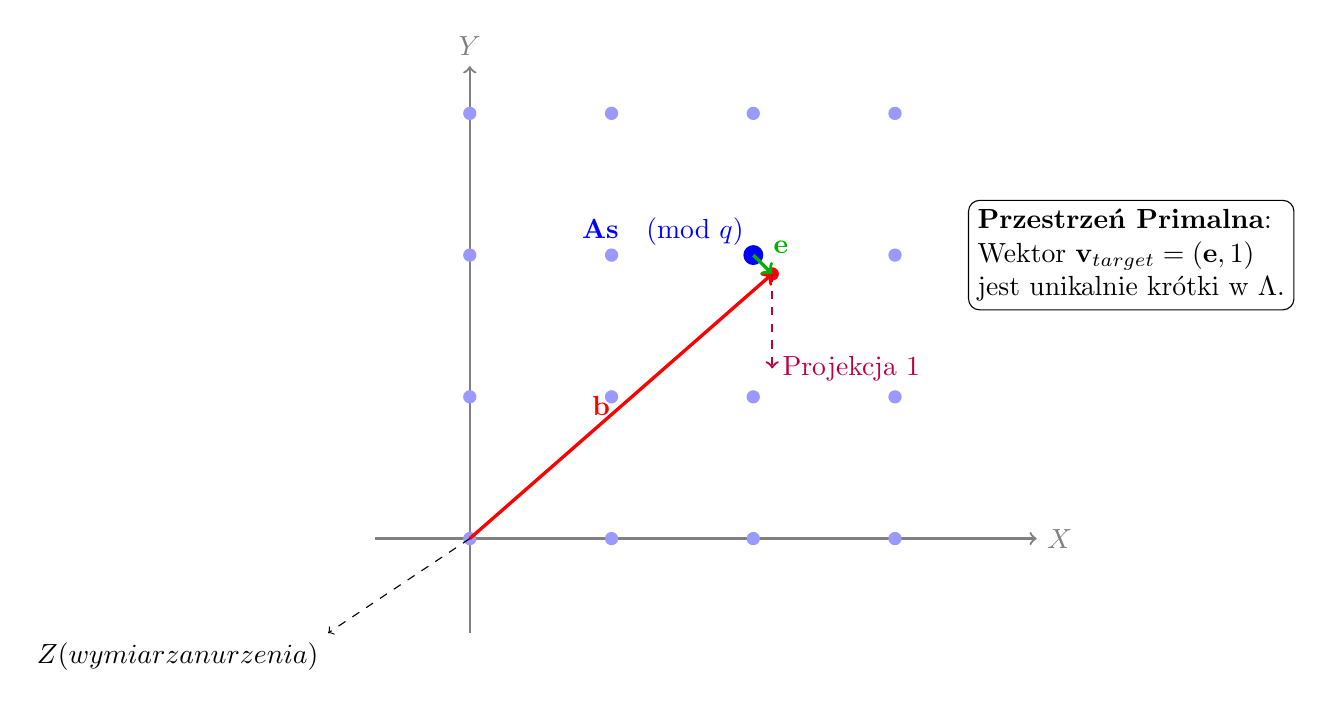
\begin{tikzpicture}[scale=1.2]
        % Osie
        \draw[->, thick, gray] (-1,0) -- (6,0) node[right] {$X$};
        \draw[->, thick, gray] (0,-1) -- (0,5) node[above] {$Y$};
        
        % Punkty kraty L_q (generowane przez A i qI)
        \foreach \x in {0,1.5,...,4.5}
            \foreach \y in {0,1.5,...,4.5}
                \fill[blue!40] (\x,\y) circle (2pt);
        
        % Wektor b (cel)
        \coordinate (B) at (3.2, 2.8);
        \draw[->, red, very thick] (0,0) -- (B) node[midway, left] {$\mathbf{b}$};
        \fill[red] (B) circle (2pt);
        
        % Najbliższy punkt kraty As
        \coordinate (AS) at (3, 3);
        \fill[blue] (AS) circle (3pt) node[above left] {$\mathbf{As} \pmod q$};
        
        % Wektor błędu e
        \draw[->, green!70!black, very thick] (AS) -- (B) node[midway, above right] {$\mathbf{e}$};
        
        % Oś Z dla zanurzenia
        \draw[->, dashed] (0,0) -- (-1.5, -1) node[below left] {$Z \text{ (wymiar zanurzenia)}$};
        
        % Wektor v_target w wyższym wymiarze
        \node[align=left, draw, rectangle, rounded corners] at (7, 3) {
            \textbf{Przestrzeń Primalna}: \\
            Wektor $\mathbf{v}_{target} = (\mathbf{e}, 1)$ \\
            jest unikalnie krótki w $\Lambda$.
        };
        
        \draw[->, purple, thick, dashed] (B) -- ++(0, -1) node[right] {Projekcja $1$};
    \end{tikzpicture}
    \caption{Schematyczna reprezentacja redukcji problemu. W przestrzeni $\mathbb{Z}_q^m$ wektor $\mathbf{b}$ nie należy do kraty generowanej przez $\mathbf{A}$. Różnica ta stanowi wektor błędu $\mathbf{e}$. W kracie primalnej (o wymiarze $m+n+1$), wektor łączący $\mathbf{b}$ i $\mathbf{As}$ staje się elementem bazy.}
\end{figure}
